\chapter{Simulación y validación del modelo}
\label{cap:capitulo5}

\vspace{0.25cm}

\section{Introducción}
\label{sec:segundaseccion}

Una vez desarrollado el modelo cinemático del CDPR, se ha llevado a cabo un proceso de validación y simulación con el objetivo de comprobar las expresiones matemáticas obtenidas del modelo cinemático en una primera implementación software. Esto permite verificar el comportamiento del sistema para así poder detectar posibles errores de planteamiento y evitar que se vayan acarreando a la hora de integrar el sistema completo en ROS 2.

\vspace{0.25cm}

En el caso de este TFG, las pruebas del modelo cinemático se han ido realizando de forma progresiva mediante su implementación en tres lenguajes de programación diferentes: MATLAB, Python y C++.

\section{Simulación inicial en MATLAB}
\label{sec:segundaseccion}

MATLAB es el primer lenguaje de programación que se ha utilizado para validar el modelo cinemático, ya que éste se considera idóneo para tratar expresiones matemáticas y obtener una rápida visualización de los resultados. Es por ello que, en esta fase inicial, la simulación se ha centrado exclusivamente en verificar que el efector final se ubica correctamente en una posición $(x,y)$ específica.

\vspace{0.25cm}

Esta primera implementación permite introducir directamente la posición $(x,y)$ en la que se quiere mostrar el efector final, además de ofrecer una representación gráfica de su posición exacta dentro del espacio de trabajo junto con toda la estructura del sistema y la disposición de los cables. 

\begin{figure} [h!]
    \begin{center}
        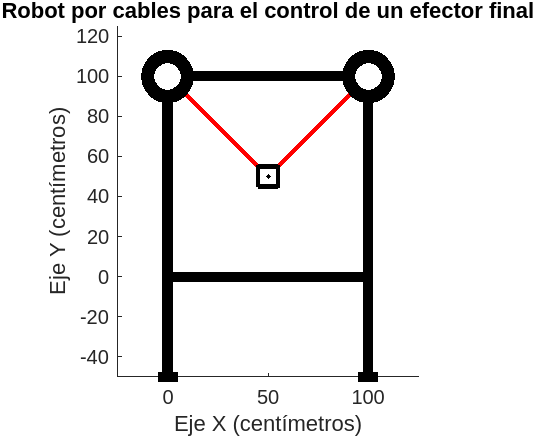
\includegraphics[width=0.5\textwidth]{figs/matlab_kinematic_model.png}
    \end{center}
    \caption{Simulación inicial en MATLAB}
\end{figure}\

\newpage

Con esto se ha cumplido el objetivo de esta primera versión, que no comprende la simulación del movimiento del efector final ni la planificación de trayectorias, sino que lo que se busca es verificar que el modelo cinemático sitúe al efector final en la posición deseada y que las longitudes de los cables calculadas sean coherentes con la geometría del sistema, sirviendo así como validación conceptual del modelo y como punto de partida para implementaciones posteriores.

\section{Implementación del modelo en Python}
\label{sec:segundaseccion}

Una vez validado el primer modelo en MATLAB, se ha desarrollado una implementación más avanzada en Python, la cual ya incluye animaciones y la posibilidad de definir múltiples posiciones objetivo para así generar trayectorias contínuas que conecten dichos puntos.

\vspace{0.25cm}

Esta segunda implementación permite introducir una secuencia de posiciones objetivo para el efector final dentro del espacio de trabajo. A partir de estas posiciones, se pueden interpolar trayectorias rectilíneas entre puntos consecutivos, mientras se calculan en cada instante las longitudes y los ángulos de cada cable utilizando las ecuaciones correspondientes de cinemática inversa.

\newpage

Además, esta implementación incluye una representación gráfica del sistema, en la que se muestra la estructura, la trayectoria realizada, y la variación del movimiento del efector final y los cables en todo momento, facilitando así la comprensión del funcionamiento del sistema y permitiendo observar de forma intuitiva cómo va evolucionando el movimiento del efector final y de los cables. Es por ello que esta segunda versión ya se aproxima mucho más al funcionamiento que se implementará posteriormente en ROS 2.

\vspace{0.25cm}

Para una mejor comprensión del comportamiento dinámico del sistema mostrado en la figura, se adjunta un enlace de descarga a un vídeo demostrativo al que se puede acceder haciendo clic \href{https://github.com/aleon2020/cable_driven_parallel_robot_2d/raw/refs/heads/main/media/gifs/python_kinematic_model_v3_execution.gif}{aquí}.

\begin{figure} [h!]
    \begin{center}
        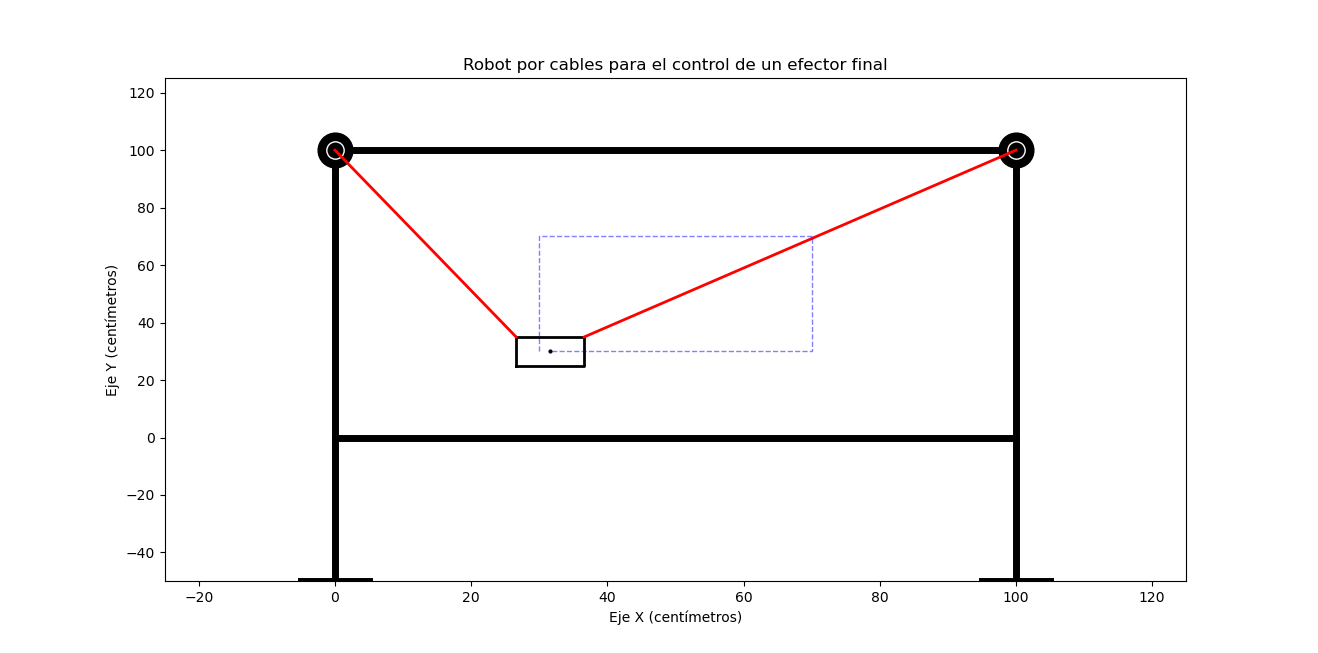
\includegraphics[width=0.5\textwidth]{figs/python_kinematic_model_v3.png}
    \end{center}
    \caption{Implementación y simulación en Python}
\end{figure}\

\section{Implementación del modelo en C++}
\label{sec:segundaseccion}

En paralelo a la implementación en Python, se ha desarrollado una versión del modelo cinemático en C++. Esta implementación reproduce la misma lógica que la vista en Python, permitiendo la definición de varias posiciones objetivo y el cálculo de la longitud de los cables en cada momento para recorrer una trayectoria.

\vspace{0.25cm}

Esta simulación se ha llevado a cabo únicamente con fines de verificación y comparación para asegurar que el modelo cinemático es independiente del lenguaje de programación utilizado, y que todas las ecuaciones que lo forman sean consistentes. Y aunque la visualización gráfica en C++ no sea tan completa como la de Python, también es útil para validar todos los cálculos numéricos realizados.

\vspace{0.25cm}

Para una mejor comprensión del comportamiento dinámico del sistema mostrado en la figura, se adjunta un enlace de descarga a un vídeo demostrativo al que se puede acceder haciendo clic \href{https://github.com/aleon2020/cable_driven_parallel_robot_2d/raw/refs/heads/main/media/gifs/cpp_kinematic_model_v3_execution.gif}{aquí}.

\begin{figure} [h!]
    \begin{center}
        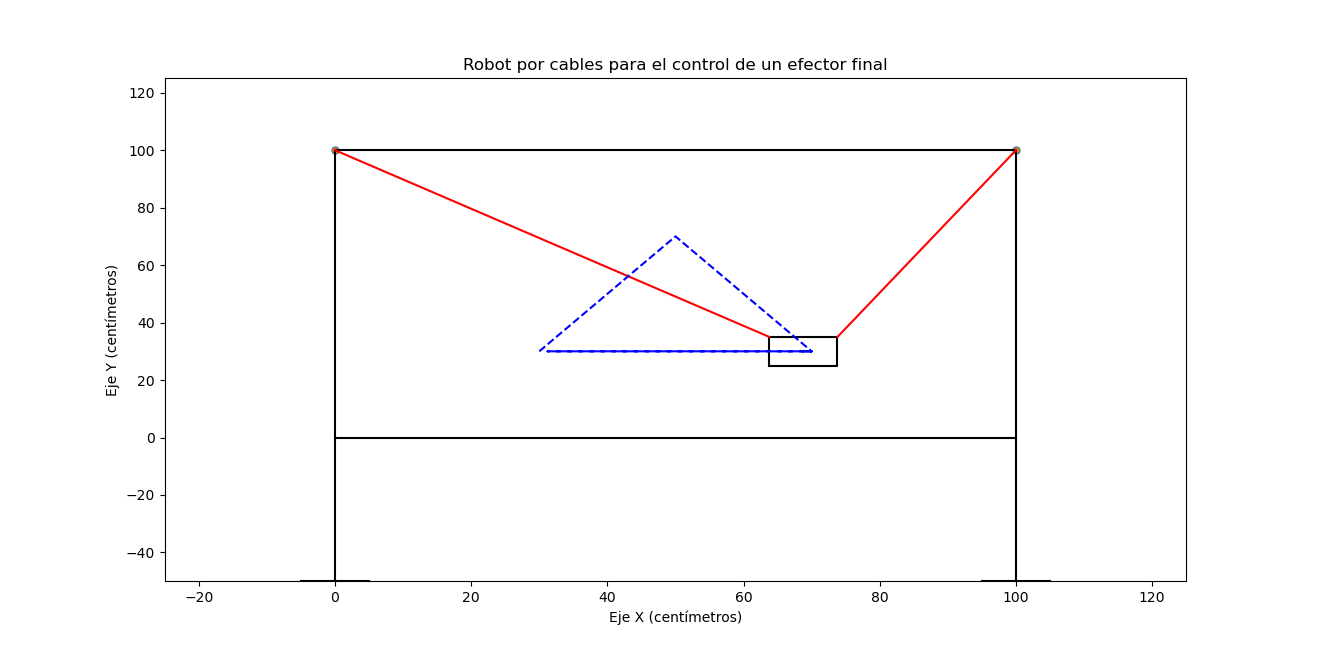
\includegraphics[width=0.5\textwidth]{figs/cpp_kinematic_model_v3.png}
    \end{center}
    \caption{Implementación y simulación en C++}
\end{figure}\

\section{Comparación y validación de resultados}
\label{sec:segundaseccion}

Para validar el modelo cinemático, se han comparado los resultados obtenidos en las tres implementaciones, y todas ellas presentan una muy buena concordancia, lo que deja más que confirmado que el modelo cinemático utilizado es totalmente correcto.

\vspace{0.25cm}

Sin embargo, existen algunas diferencias en cuanto a funcionalidad y flexibilidad. MATLAB se ha utilizado como herramienta para llevar a cabo una primera validación, limitándose únicamente al posicionamiento de una única posición objetivo, mientras que las implementaciones realizadas en Python y en C++ permiten la generación de trayectorias definidas por múltiples posiciones objetivo.

\vspace{0.25cm}

Y es por eso que, tras este análisis comparativo, he decidido utilizar Python como lenguaje principal a la hora de implementar el sistema en ROS 2, debido a la facilidad que supone desarrollar en Python ofreciendo la posibilidad de poder integrarlo directamente en ROS 2, manteniendo el mismo comportamiento cinemático que en C++.

\section{Análisis de errores y limitaciones}
\label{sec:segundaseccion}

Durante el proceso de simulación, se han identificado algunas limitaciones que no afectan al sistema debido al enfoque que se le ha dado al mismo, ya que al tratarse de un modelo puramente cinemático, no se consideran efectos dinámicos como la masa del efector final, la elasticidad de los cables o la fricción de las poleas.

\vspace{0.25cm}

Por otro lado, todas las simulaciones se realizan en lazo abierto, lo que implica que todos los resultados obtenidos dependen directamente de la precisión del modelo y de los parámetros geométricos definidos. Todas estas limitaciones no invalidan ningún aspecto del sistema ya definido, pero es importante tenerlas en cuenta a la hora de interpretar los resultados cuando se esté implementando en un entorno físico real.
